\section{Partitionen}
\begin{frame}{Partition}
 \begin{itemize}
  \item Träger von Filesystemen
  \item Aufbau
  \begin{itemize}
   \item MBR: Master Boot Record
  \end{itemize}
  \item Herstellung
 \end{itemize}
 \remark{Alles ist ein File  {\em stream of bits}}
\end{frame}

\subsection{Massenspeicher}
\begin{frame}{Massenspeicher}{non volatile}
 \begin{block}{Arten}
  \begin{itemize}
   \item mechanische Festplatten
   \item SSD Karten
   \item SD-Karten
   \item Flash
   \item ...
  \end{itemize}
 \end{block}
 \begin{block}{Typisch}
  \begin{itemize}
   \item Zugriff relativ langsam
   \item Blockorientiert 
   \begin{itemize}
    \item Mehrere Bits/Bytespro Zugriff
   \end{itemize}
  \end{itemize}
 \end{block}
\end{frame}


\begin{frame}{Partitionen Termiologie \linux}{Träger von Filesystemen}
  \begin{itemize}
   \item Massenspeicher
   \begin{itemize}
   \item \cod{/dev/sd{\em X}}, \cod{{\em X}=a,b,c ...}
   \end{itemize} 
   \item Partitionen 
   \begin{itemize}
     \item \cod{/dev/sd{\em X}{\em N}} \cod{{\em N}=1,2,3 ...} 
   \end{itemize} 
  \end{itemize}
  \begin{block}{\Huge Vorsicht}
   \begin{itemize}
    \item Festplatte vom \host ist auch ein \cod{/dev/sd{\em X}}
   \end{itemize}
  \end{block}
\end{frame} 


\begin{frame}[fragile]{Massenspeicher}{Blocks/Sektoren}
\begin{lstlisting}
 typedef unsigned char Sector[512]; 
 Sector MassStorage[N];
\end{lstlisting}
\remark{Ein langer Array von Sektoren}
\begin{center}
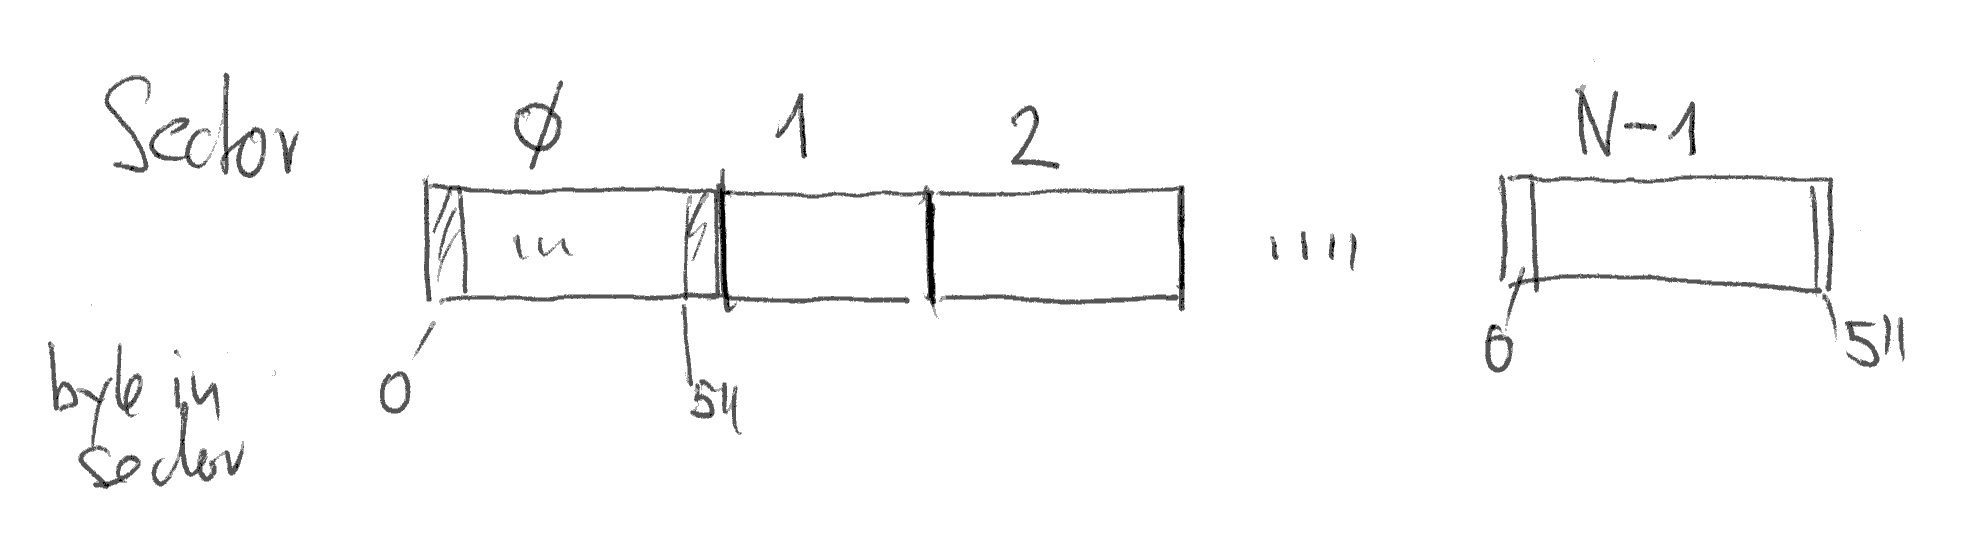
\includegraphics[width=0.875\textwidth]{array-of-sector.jpg}
\end{center}
\end{frame}

\begin{frame}[fragile]{Der Befehl \cod{dd}}{Vorsicht}
\begin{lstlisting}[language=bash]
dd if=/dev/sdX count=1|hexdump -C        
  # first sector to stdout
dd if=/dev/sdX skip=1 count=1|hexdump -C 
  # second sector to stdout
dd if=/dev/sdX of=mbr.bin count=1        
  # copy sector to mbr.bin
\end{lstlisting}
  \begin{block}{\Huge Vorsicht}
   \begin{itemize}
    \item Festplatte vom \host ist auch ein \cod{/dev/sd{\em X}}
   \end{itemize}
  \end{block}

\end{frame}

\subsection{MBR}
\begin{frame}[fragile]{MBR: Master Boot Record}{Verzeichnis der Partionen}
\begin{lstlisting}[language=bash]
dd if=/dev/mmcblk0 count=1|hexdump -C
\end{lstlisting}
{\scriptsize
\begin{verbatim}
00000000  00 00 00 00 00 00 00 00  00 00 00 00 00 00 00 00  |................|
*
000001b0  00 00 00 00 00 00 00 00  ba 23 8e d6 00 00 00 00  |.........#......|
000001c0  01 20 0b 03 10 1f 00 08  00 00 00 00 04 00 00 00  |. ..............|
000001d0  01 20 83 03 50 df 00 08  04 00 00 70 71 00 00 00  |. ..P......pq...|
000001e0  00 00 00 00 00 00 00 00  00 00 00 00 00 00 00 00  |................|
000001f0  00 00 00 00 00 00 00 00  00 00 00 00 00 00 55 aa  |..............U.|
00000200
\end{verbatim}
}

{\scriptsize\url{technet.microsoft.com/en-us/library/cc976786.aspx}}

\end{frame}

